% Created 2017-07-07 Fri 23:36
% Intended LaTeX compiler: pdflatex
\documentclass[11pt]{article}
\usepackage[utf8]{inputenc}
\usepackage[T1]{fontenc}
\usepackage{graphicx}
\usepackage{grffile}
\usepackage{longtable}
\usepackage{wrapfig}
\usepackage{rotating}
\usepackage[normalem]{ulem}
\usepackage{amsmath}
\usepackage{textcomp}
\usepackage{amssymb}
\usepackage{capt-of}
\usepackage{hyperref}
\author{zcl.space}
\date{}
\title{高斯随机变量}
\hypersetup{
 pdfauthor={zcl.space},
 pdftitle={高斯随机变量},
 pdfkeywords={probability},
 pdfsubject={},
 pdfcreator={Emacs 25.2.1 (Org mode 9.0.9)},
 pdflang={English}}
\begin{document}

\maketitle
\tableofcontents
\titlepic{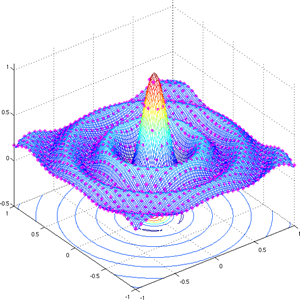
\includegraphics[scale=0.25]{../../img/sinc.PNG}}
\href{afcp-normal-distribution-history.org}{八卦一下} ,高斯随机变量不是高斯发现的,是一个叫亚伯拉罕\(\cdot\)棣莫弗的数学家发现的。无论哪个发现的高斯随机变量,都不影响高斯随机变量在概率论中的重要地位。

\section{定义}
\label{sec:org0d4ea1f}


如果随机变量\(X\)的概率密度函数是:
\begin{equation}
\label{eq:1}
f(x) = \frac{1}{\sqrt{2\pi \sigma^{2}}}e^{-\frac{(x-\mu)^{2}}{2\sigma^{2}}}, -\infty < x < \infty
\end{equation}
称这个随机变量服从参数为\(\mu\)和\(\sigma^{2}\)的高斯分布。稍后我们会发现\(\mu\)和\(\sigma^{2}\)在完全控制一个高斯变量,他们分别是该高斯变量的均值和方差。无论\(\mu\)和\(\sigma^{2}\)的值如何变化,高斯随机变量的图形始终是钟形。如图所示。

\begin{figure}[htbp]
\centering
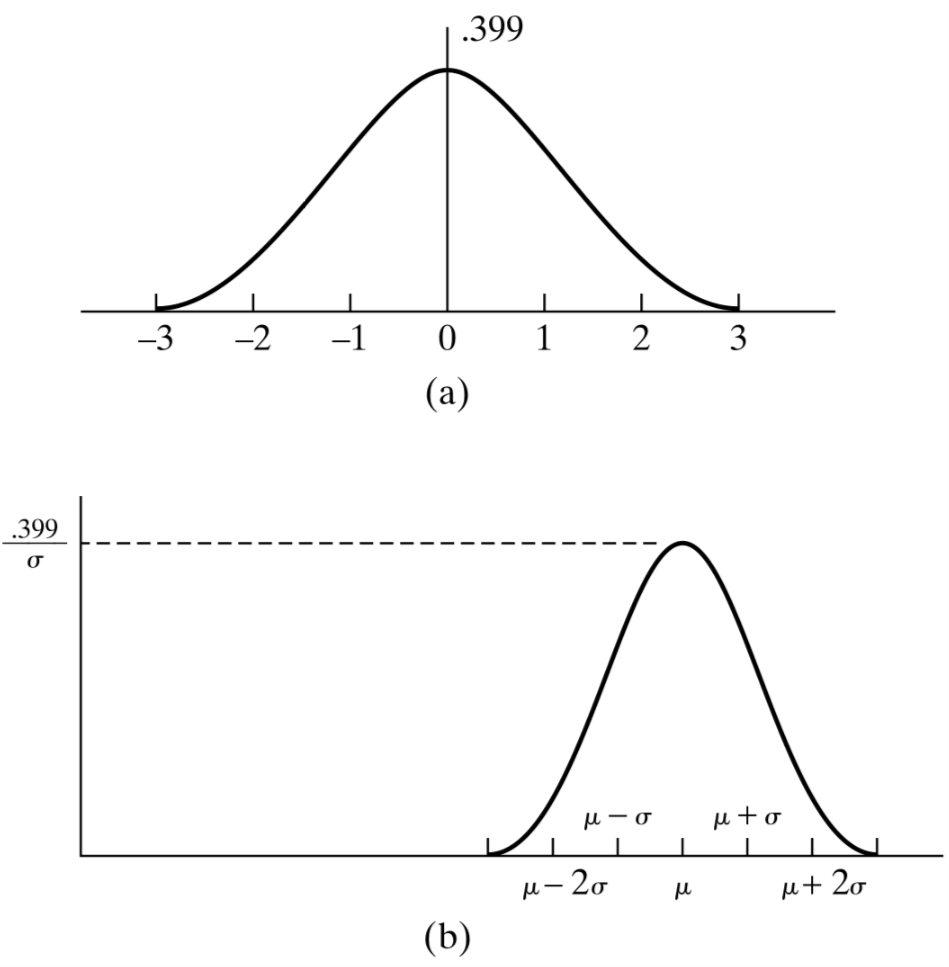
\includegraphics[width=0.6\textwidth]{../../img/math_probability/20170610figure5dot5gaussian.png}
\caption{\label{fig:org32b3e17}
高斯随机变量的形状}
\end{figure}

\(f(x)\)是一个概率密度函数,我们可以通过\(\int_{-\infty}^{\infty}f(x)dx = 1\)来验证。
\begin{equation}
\label{eq:2}
\frac{1}{\sqrt{2\pi}\sigma}\int_{-\infty}^{\infty} e^{-\frac{(x-\mu)^{2}}{2\sigma^{2}}}dx = 1
\end{equation}
变量替换,令\(y = \tfrac{x-\mu}{\sigma}\),式 (\ref{eq:2})可以变为:
\begin{equation}
\label{eq:3}
\frac{1}{\sqrt{2\pi}}\int_{-\infty}^{\infty} e^{-y^{2}/2}dy = 1
\end{equation}
即,我们需要证明
\begin{equation}
\label{eq:4}
\int_{-\infty}^{\infty} e^{-y^{2}/2}dy = \sqrt{2\pi}
\end{equation}
这个积分非常有意思,令\(I = \int_{-\infty}^{\infty} e^{-y^{2}/2}dy\),则:
\begin{equation}
\label{eq:5}
I^{2} = \int_{-\infty}^{\infty} e^{-y^{2}/2}dy \int_{-\infty}^{\infty} e^{-x^{2}/2}dx
\end{equation}
我们利用左边变换来求解上面的二重积分,令:
\begin{eqnarray}
\label{eq:6}
x&=&r\cos\theta \\
y&=&r\sin\theta
\end{eqnarray}
则\(dxdy = rd\theta dr\),所以有:
\begin{equation}
\label{eq:7}
I^{2} = \int_{0}^{\infty}\int_{0}^{2\pi}e^{-r^{2}/2}rd\theta dr = 2\pi \int_{0}^{\infty}re^{-r^{2}/2}dr = 2\pi
\end{equation}
因此\(I = \sqrt{2\pi}\)
\section{正态分布的性质}
\label{sec:orgb4a55f7}


\subsection{期望和方差}
\label{sec:orgd1a7ff1}

先从标准正态分布的期望和方差开始,由于:
\begin{equation}
\label{eq:8}
E[X] = \frac{1}{\sqrt{2\pi}}\int_{-\infty}^{\infty} xe^{-x^{2}/2}dx = 0
\end{equation}
\begin{equation}
\label{eq:9}
\mathrm{Var}[X] = \frac{1}{\sqrt{2\pi}}\int_{-\infty}^{\infty} x^{2} e^{-x^{2}/2}dx
\end{equation}
分部积分,我们得到\(\mathrm{Var}(X) = 1\)
\subsection{正态分布的线性函数}
\label{sec:org80480d4}


如果\(X\)是一个服从参数为\(\mu\)和\(\sigma^{2}\)的正态分布的随机变量,那么\(aX + b\)也服从正态分布,且参数为\(a\mu + b\)和\(a^{2}\sigma^{2}\)。设\(F_{Y}\)为\(Y\)的分布函数,则:
\begin{equation}
\label{eq:10}
F^{Y}(x) = P\{Y\leq x\} = P\{ aX + b \leq x\} = P\{ X \leq \frac{x-b}{a}\} = F_{x}(\frac{x-b}{a})
\end{equation}
其中\(F_{X}(x)\)为\(X\)的分布函数,求导可得\(Y\)的密度函数:
\begin{eqnarray}
\label{eq:11}
f_{Y}(x)&=& \frac{1}{a}f_{x}(\frac{x-b}{a}) \\
&=& \frac{1}{\sqrt{2\pi}a\sigma}e^{-\frac{ (\frac{x-b}{a}-\mu)^{2} }{2\sigma^{2}}} \\
&=& \frac{1}{\sqrt{2\pi}a\sigma}e^{-\frac{(x-b-a\mu)^{2}}{2(a\sigma)^{2}}}
\end{eqnarray}
即,假设\(X\)是均值为\(\mu\)方差为\(\sigma^{2}\)的高斯变量,则\(aX + b\)则是一个均值为\(a\mu + b\)方差为\(a^{2}\sigma^{2}\)的高斯变量。这个结论的一个重要应用是,如果\(X\)是一个参数为\(\mu,\sigma^{2}\)的正态随机变量,那么\(Z = \tfrac{X-a}{\sigma}\)是一个参数为\((0,1)\)的正态随机变量。参数为\((0,1)\)的正态随机变量成为标准正态随机变量。
\section{棣莫弗拉普拉斯极限定理}
\label{sec:org7b5385f}


概率论中一个重要的结论就是棣莫弗拉普拉斯极限定理,它表明当\(n\)充分大时,参数为\(n,p\)的二项随机变量可以由正态随机变量来近似,其中正态随机变量的期望和方差与二项随机变量的期望和方差相同。更一般的表述:我们可以将二项随机变量标准化,先减去均值\(np\),然后再除以标准差\(\sqrt{np(1-p)}\),那么经过标准化后的随机变量的分布函数当\(n\to \infty\)时收敛于标准正态分布。

\begin{tikztheorem}[棣莫弗拉普拉斯定理]
在\(n\)次独立重复试验中,设每次成功的概率为\(p\),记成功的总次数为\(S_{n}\),那么对于任意\(a < b\)有:当(n\(\to\) \(\infty\))时,
\begin{equation}
\label{eq:12}
P\bigg\{a\leq \frac{S_{n}-np}{\sqrt{np(1-p)}} \leq b\bigg\} \to \Phi(b) - \Phi(a)
\end{equation}
\end{tikztheorem}

现在,二项分布有两种可能的近似:当\(n\)较大\(p\)较小时,\href{poisson-distribution.org}{泊松分布} 是一个很好的近似;另外,可以证明,当\(np(1-p)\)较大时,正态分布近似的效果很好。一般情况下,当\(np(1-p) \geq 10\)时,正态近似就非常好。
\end{document}
